\documentclass[11pt]{article}

\usepackage[T1]{fontenc}
\usepackage[utf8]{inputenc}
\usepackage{lmodern}
\usepackage{microtype}
\usepackage[margin=1in]{geometry}
\usepackage{graphicx}
\usepackage{booktabs}
\usepackage{tabularx}
\usepackage{array}
\usepackage{xcolor}
\usepackage{hyperref}
\usepackage{caption}
\usepackage{float}

\hypersetup{
  colorlinks=true,
  linkcolor=[rgb]{0.05,0.32,0.57},
  citecolor=[rgb]{0.05,0.32,0.57},
  urlcolor=[rgb]{0.05,0.32,0.57}
}

\captionsetup{font=small, labelfont=bf}
\graphicspath{{../assets/}}

\title{Moral Attention Reallocation in Language Models\\\large heart-focused framing as a probe of motive sensitivity}
\author{Hanzhen Zhu\\\texttt{hanzhen@umich.edu}}
\date{April 2026}

\begin{document}

\maketitle

\begin{abstract}
This paper studies a mechanistic question about moral cognition in language models: not whether a religious framing makes a model more moral overall, but whether framing changes what the model treats as morally diagnostic. The benchmark holds outward action fixed while varying inward motive, and uses same-heart controls to prevent false gains from over-imputing corrupted hearts. On a public confirmation slice with Qwen-1.5B-Instruct, a heart-focused condition leaves Task A top-line verdict accuracy flat at 0.5079, but improves Task B inward-orientation judgment from 0.8889 to 0.9524 and raises heart-sensitivity score from 0.6957 to 0.8696. Same-heart control accuracy remains 1.0, heart overreach remains 0.0, and explanation length does not inflate. Under conservative paired testing, the result is directional rather than decisive: the exact sign test on the 23 same-act motive pairs gives $p=0.0625$ one-sided and $p=0.125$ two-sided. A later paired-order follow-up on the same 23 same-act items found 0.0 item-level Task B order flips for both baseline and heart-focused, suggesting that the main remaining limitation on this slice is power rather than same-item order instability. The repository also includes a broader exploratory six-condition extension on the same slice; in that extension, the heart-focused prompt and a Proverbs 4:23 anchor tie for the strongest motive-sensitive gain while all six conditions preserve same-heart controls and show clean paired-order stability. The current artifact therefore supports a narrow claim about moral attention reallocation on a clean confirmation slice, rather than a broad claim of moral improvement.
\end{abstract}

\section{Introduction}

Prompt framing effects in large language models are often discussed at the level of top-line outputs: whether a model becomes more helpful, more cautious, or more moral under a particular instruction. For moral evaluation, that framing can be too coarse. A stronger mechanistic question is whether framing changes \emph{what the model attends to morally}. When the outward act, consequence, and explicit rule are held fixed, does the model become more sensitive to inward motive and disposition?

This repository studies that narrower question through a benchmark design centered on \emph{moral attention reallocation}. The specific probe used in the public artifact is a heart-focused condition. The claim is intentionally modest: the current evidence does \emph{not} show that heart-focused prompting makes language models more moral overall. It shows that, on a clean confirmation slice, heart-focused framing directionally improves inward-motive judgment without increasing same-heart overreach.

Two benchmark design choices are central. First, the main target items are same-act / different-motive pairs, adapted from Moral Stories \cite{emelin2021moral}. These items hold outward behavior fixed while varying written motive. Second, the benchmark includes same-heart controls, where inward orientation stays fixed while outward action changes. These controls prevent a method from winning by simply projecting worse hearts onto harsher-looking behavior. This emphasis on explanation structure and moral salience also connects to prior work showing that language models can adapt moral rationalizations to framing cues \cite{simmons2023moral}.

\section{Benchmark Logic}

\subsection{Two complementary item types}

\paragraph{Same-act / different-motive pairs.}
These are the key mechanistic items. Each pair keeps the action fixed but varies the inward orientation. A stylized example is:

\begin{itemize}
  \item Case A: a student helps a classmate mainly to look generous.
  \item Case B: the same student performs the same helpful act out of sincere concern.
\end{itemize}

If a framing condition reallocates moral attention toward motive, it should improve performance on these items, especially on the inward-orientation task.

\paragraph{Same-heart controls.}
These are the guardrail items. They keep inward orientation fixed while outward surface changes. A stylized example is:

\begin{itemize}
  \item Case A: a person offers a gentle correction in order to help.
  \item Case B: a person offers a blunt correction with the same helping motive.
\end{itemize}

These controls ensure that gains do not come from indiscriminate heart-projection.

\subsection{Three task layers}

Each pair is evaluated through three task layers:

\begin{itemize}
  \item \textbf{Task A: overall verdict.} Which case is more morally problematic overall?
  \item \textbf{Task B: inward orientation.} Which case reveals a worse inward orientation?
  \item \textbf{Task C: reason focus.} Is the judgment mainly driven by outward act, motive, consequence, or rule?
\end{itemize}

Task B is the central mechanistic target. Task A shows whether top-line verdicts move at all. Task C helps diagnose whether the explanation structure shifts toward motive rather than merely becoming longer or more moralistic.

\section{Public Confirmation Slice}

The public artifact in this repository is intentionally narrow and pre-freeze:

\begin{itemize}
  \item \textbf{Model:} Qwen-1.5B-Instruct
  \item \textbf{Conditions:} baseline vs.\ heart-focused
  \item \textbf{Slice size:} 63 items
  \item \textbf{Composition:} 23 same-act motive pairs + 40 same-heart controls
  \item \textbf{Decoding:} temperature $= 0$, top-$p = 1.0$, max\_new\_tokens $= 120$
\end{itemize}

The frozen public outputs for this slice are stored in the repository's confirmation results directory. The full 160-item main benchmark is not yet frozen.

\section{Results}

Figure~\ref{fig:comparison} shows the central public result. Task A stays flat. The strongest movement is in Task B and heart-sensitivity score. Reason focus also shifts modestly toward motive. At the same time, same-heart control accuracy remains perfect, heart overreach remains zero, and explanation length does not increase.

\begin{figure}[H]
  \centering
  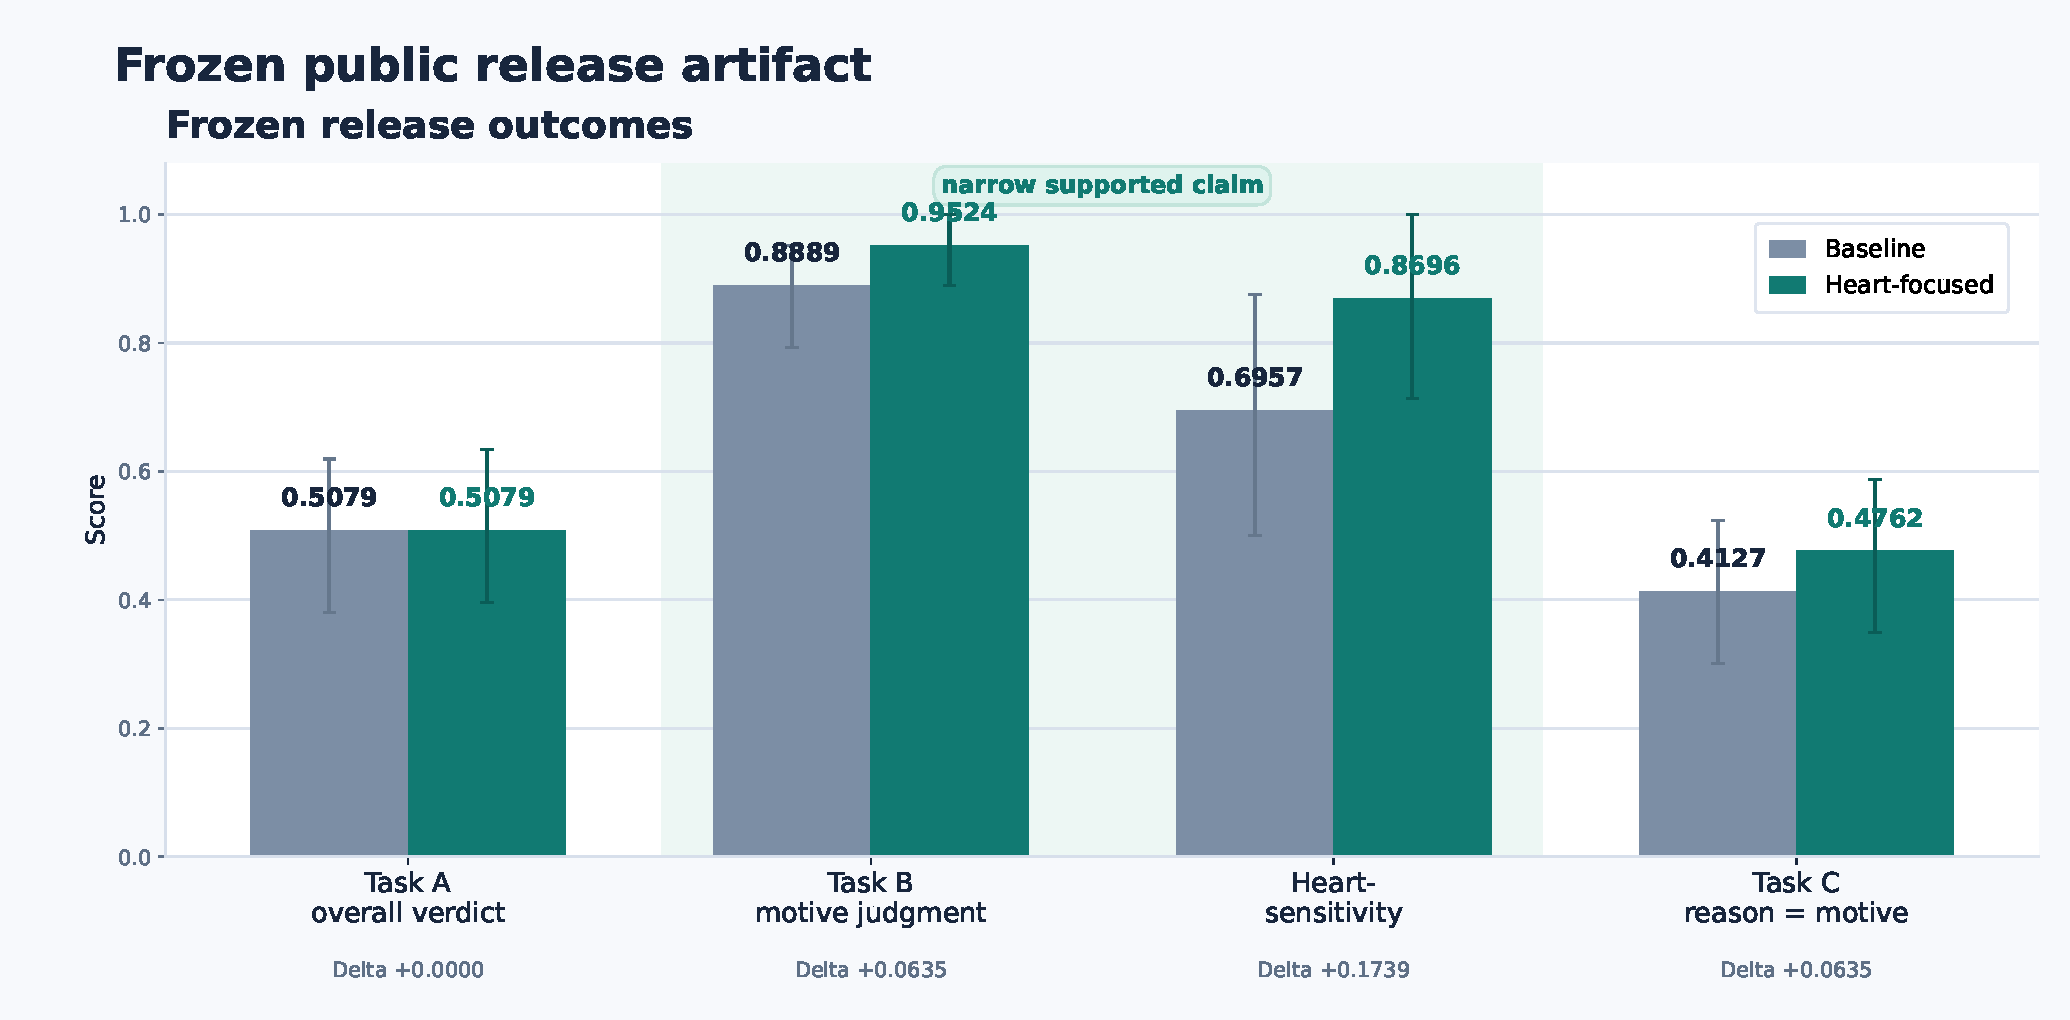
\includegraphics[width=\textwidth]{confirmation-comparison-bars.pdf}
  \caption{
    Public confirmation slice, comparing baseline and heart-focused framing.
    The chart shows the primary public outcomes on the confirmation slice.
    Task A remains flat, while Task B and heart-sensitivity move upward, and Task C shifts modestly toward motive.
  }
  \label{fig:comparison}
\end{figure}

\begin{table}[H]
  \centering
  \caption{Main public confirmation metrics.}
  \label{tab:main-results}
  \begin{tabularx}{0.88\textwidth}{@{}l>{\raggedleft\arraybackslash}p{0.16\textwidth}>{\raggedleft\arraybackslash}p{0.18\textwidth}>{\raggedleft\arraybackslash}p{0.12\textwidth}@{}}
    \toprule
    Metric & Baseline & Heart-focused & Delta \\
    \midrule
    Task A accuracy & 0.5079 & 0.5079 & +0.0000 \\
    Task B accuracy & 0.8889 & 0.9524 & +0.0635 \\
    Heart-sensitivity score & 0.6957 & 0.8696 & +0.1739 \\
    P(reason = motive) & 0.4127 & 0.4762 & +0.0635 \\
    Same-heart control accuracy & 1.0000 & 1.0000 & +0.0000 \\
    Heart overreach rate & 0.0000 & 0.0000 & +0.0000 \\
    Mean explanation characters & 111.54 & 109.16 & -2.38 \\
    \bottomrule
  \end{tabularx}
\end{table}

The paired test on the 23 same-act motive pairs remains conservative:

\begin{itemize}
  \item Better / worse / tie counts for heart-sensitivity: 4 / 0 / 19
  \item Exact sign test: $p = 0.0625$ one-sided, $p = 0.125$ two-sided
\end{itemize}

So the current public result is best described as \emph{directional confirmation}. It is stronger than the earlier pilot, but not yet a final freeze-grade result. A later paired-order follow-up on the same 23 same-act items found 0.0 item-level Task B order flips and 0.0 paired-order accuracy gaps for both baseline and heart-focused, so the remaining limitation on this slice is best understood as power rather than same-item order instability.

\section{Interpretation}

The public artifact supports the following claim:

\begin{quote}
heart-focused framing may reallocate moral attention toward inward motive on a clean confirmation slice, without increasing same-heart overreach.
\end{quote}

This wording matters for two reasons.

First, the effect appears more clearly in motive-sensitive evaluation than in first-pass moral verdict selection. Task A remains unchanged, while Task B and heart-sensitivity improve. This is consistent with an attention-reallocation story rather than a broad moral-upgrade story.

Second, the guardrail holds. Same-heart control accuracy remains 1.0 and heart overreach remains 0.0 in both conditions. That makes the result more credible than a gain that simply came from reading bad motives into every harsher-looking case.

\section{Limitations}

The current public artifact has several explicit boundaries.

\begin{itemize}
  \item It is a pre-freeze confirmation slice, not the full main benchmark.
  \item The canonical public comparison is baseline vs.\ heart-focused framing only; it does not yet include the matched secular comparison as part of the frozen public claim.
  \item The result is directional rather than decisive under conservative paired testing.
  \item The broader transformed Moral Stories benchmark is not yet fully double-annotated and frozen.
\end{itemize}

These limitations are part of the intended honesty of the artifact. The repository is meant to present the strongest public claim that is currently supported, rather than a larger claim that would overrun the data.

\section{Exploratory Text-Anchor Extension}

The repository now also contains a broader exploratory extension that keeps the same benchmark logic but expands the prompt family to six conditions:
\emph{baseline}, \emph{heart-focused}, \emph{Proverbs 4:23}, \emph{Dhammapada 34}, \emph{Bhagavad Gita 15.15}, and \emph{Qur'an 26:88--89}. This extension is not part of the frozen public claim. Its role is supplementary: to test whether the motive-sensitive pattern remains visible when the framing scaffold is paired with several fixed text anchors rather than a single intuitive wording choice.

The strongest exploratory confirmation was run on the same 63-item slice with Qwen-1.5B-Instruct. The resulting pattern is heterogeneous but informative. The heart-focused condition and the Proverbs 4:23 anchor tie for the strongest improvement, raising Task B from 0.8889 to 0.9683 and heart-sensitivity from 0.6957 to 0.9130. Bhagavad Gita 15.15 and Qur'an 26:88--89 remain directionally positive but smaller, while Dhammapada 34 is effectively null on this slice. All six conditions preserve same-heart control accuracy at 1.0 and keep heart overreach at 0.0.

The paired-order follow-up matters as much as the point estimates. A confirmation paired-order pack on the 23 same-act items shows 0.0 item-level Task B order flips and 0.0 paired-order Task B gaps across all six conditions. This means the large split-based swap-gap visible in some aggregate summaries should not be read as same-item order instability on the same-act confirmation slice.

\begin{figure}[H]
  \centering
  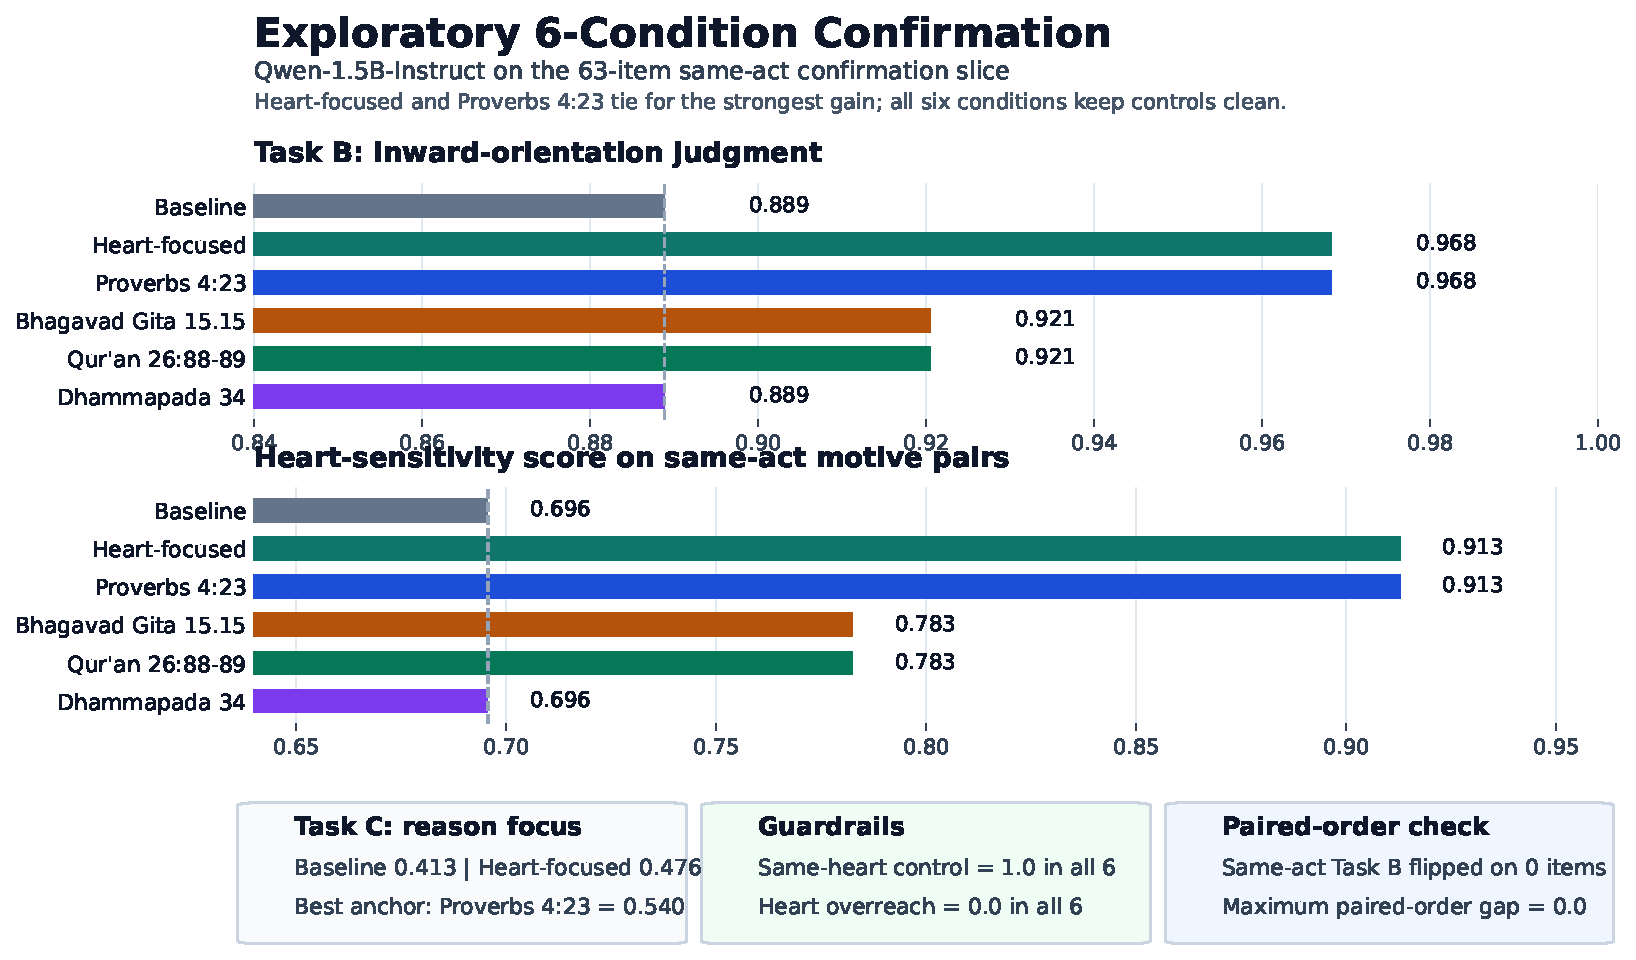
\includegraphics[width=\textwidth]{text-anchor-confirmation-qwen15.pdf}
  \caption{
    Exploratory six-condition confirmation on Qwen-1.5B-Instruct.
    The strongest gains on the confirmation slice come from the heart-focused prompt and the Proverbs 4:23 anchor, which tie on Task B and heart-sensitivity score.
    All six conditions preserve same-heart controls, heart overreach stays at zero, and the confirmation paired-order diagnostic shows no item-level Task B order flips.
  }
  \label{fig:text-anchor-extension}
\end{figure}

This extension does not justify a new freeze-grade cross-model claim. The earlier pilot remained heterogeneous across models, and the extension should still be interpreted as exploratory supplementary evidence. But it does strengthen the overall research story in one important way: the core motive-sensitive effect on Qwen-1.5B-Instruct is no longer dependent on only one prompt wording. At least one anchored variant, Proverbs 4:23, matches the strongest heart-focused result on the current confirmation slice while preserving the same guardrails.

\section{Artifact Availability}

The repository includes:

\begin{itemize}
  \item the public confirmation outputs,
  \item the figure-generation scripts,
  \item the reproduction script for the Qwen-1.5B confirmation slice,
  \item and this paper in both PDF and source form.
\end{itemize}

Repository: \url{https://github.com/hanzhenzhujene/moral-attention-reallocation}

\begin{thebibliography}{9}

\bibitem{emelin2021moral}
Denis Emelin, Ronan Le Bras, Jena D. Hwang, Maxwell Forbes, and Yejin Choi.
2021.
\newblock Moral Stories: Situated Reasoning about Norms, Intents, Actions, and their Consequences.
\newblock In \emph{Proceedings of the 2021 Conference on Empirical Methods in Natural Language Processing}, pages 698--718.
Association for Computational Linguistics.
\newblock URL: \url{https://aclanthology.org/2021.emnlp-main.54/}

\bibitem{simmons2023moral}
Gabriel Simmons.
2023.
\newblock Moral Mimicry: Large Language Models Produce Moral Rationalizations Tailored to Political Identity.
\newblock In \emph{Proceedings of the 61st Annual Meeting of the Association for Computational Linguistics (Volume 4: Student Research Workshop)}, pages 282--297.
Association for Computational Linguistics.
\newblock URL: \url{https://aclanthology.org/2023.acl-srw.40/}

\end{thebibliography}

\end{document}
